\RequirePackage{fix-cm}
\documentclass[oneside, a4paper]{book}
\usepackage[a4paper,width=150mm,top=25mm,bottom=25mm,bindingoffset=6mm]{geometry}

\title{Equation of State Solver for Smoothed Particle Hydrodynamics}
\author{Julian Karrer}

% Required for inserting images
\usepackage{eso-pic,graphicx}

% misc
\usepackage{caption}
\DeclareCaptionType{equ}[][]
%\captionsetup[equ]{labelformat=empty}

\usepackage{subcaption}
\usepackage{multicol}
\usepackage{float}
\usepackage{adjustbox} % oversized table

% Default font to sans serif
\renewcommand{\familydefault}{\sfdefault}
\RequirePackage[T1]{fontenc} 
\RequirePackage[tt=false, type1=true]{libertine} 
\RequirePackage[varqu]{zi4} 
% \RequirePackage[libertine]{newtxmath}

% chapters and headers
\usepackage[Conny]{fncychap}

\usepackage{fancyhdr}
\pagestyle{fancy}
\renewcommand{\headrulewidth}{0.1pt}
\renewcommand{\chaptermark}[1]{\markboth{\MakeUppercase{\textsf{#1}}}{}}
\renewcommand{\sectionmark}[1]{ \markright{\MakeUppercase{\textsf{\thesection\ #1}}}{} }

% algorithms
\usepackage{algorithm}
\usepackage{algpseudocode}

% FAT FONTS
\usepackage{bm} % bold fonts in math mode
\newcommand\fat[1]{{\boldmath{\textbf{#1}}}}
\newcommand\emphasis[1]{{\scshape\bfseries#1}}

% mathematical fonts and graphics
\usepackage{mathtools}
\usepackage{xfrac} % sfrac for diagonal slashes in fractions
\usepackage{amsfonts} % math fonts
\usepackage{dsfont} % math fonts
\usepackage{bbm} % mathbb fonts
\usepackage{mathrsfs} % fancy swirly font
\usepackage{gensymb} % degree sign

% draw graphs
\usepackage[inline]{asymptote}
\usepackage{qtree}
\usepackage{tikz}

% plots
\usepackage{pgfplots}
\usepgfplotslibrary{external}
\tikzexternalize
\pgfplotsset{compat=1.18} 

% get width of given text
\usepackage{calc}

% define a horizontal spacer
\newcommand\horizontalspacer[0]{\vspace{5pt}\noindent\textcolor{lightgray}{\rule{\textwidth}{1mm}}
\vspace{5pt}}

% clickable links
\usepackage{hyperref}
\hypersetup{
    colorlinks,
    citecolor=black,
    filecolor=black,
    linkcolor=black,
    urlcolor=black
}
% citations
\usepackage[
  backend=biber,
  sorting=none,
  style=phys,
]{biblatex}
\addbibresource{refs.bib}

% fancy boxes
\usepackage{fancybox}

% fancy chapter headings
\makeatletter
\def\thickhrulefill{\leavevmode \leaders \hrule height 1ex \hfill \kern \z@}
\def\@makechapterhead#1{%
  %\vspace*{50\p@}%
  \vspace*{10\p@}%
  {\parindent \z@ \centering \reset@font
        \thickhrulefill\quad
        \scshape \@chapapp{} \thechapter
        \quad \thickhrulefill
        \par\nobreak
        \vspace*{10\p@}%
        \interlinepenalty\@M
        \hrule
        \vspace*{10\p@}%
        \Huge {\textbf{#1}} \par\nobreak
        \par
        \vspace*{10\p@}%
        \hrule
    \vskip 40\p@
    % \vskip 100\p@
  }}
\def\@makeschapterhead#1{%
  %\vspace*{50\p@}%
  \vspace*{10\p@}%
  {\parindent \z@ \centering \reset@font
        \thickhrulefill
        \par\nobreak
        \vspace*{10\p@}%
        \interlinepenalty\@M
        \hrule
        \vspace*{10\p@}%
        \Huge \bfseries #1\par\nobreak
        \par
        \vspace*{10\p@}%
        \hrule
    \vskip 40\p@
    % \vskip 100\p@
  }}

  
\usepackage[pdftex,outline]{contour}

% ~~~~~~~~~ MATH MACROS ~~~~~~~~~~~~~~~~~~~~~~~~~~~~~~~~~~~~~~

% abs value macro
% \DeclarePairedDelimiter\abs{\lvert}{\rvert}
\newcommand\abs[1]{\left|#1\right|}

% define the laplace operator 
\newcommand*\Laplace{\mathop{}\!\mathbin\nabla^2}
\newcommand\vek[1]{\vec{\bm{#1}}}

\DeclareMathOperator{\sgn}{sgn}
\DeclareMathOperator{\erf}{erf}


% ~~~~~~~~~ START ~~~~~~~~~~~~~~~~~~~~~~~~~~~~~~~~~~~~~~~~~~~

\captionsetup[figure]{font=footnotesize,labelfont=footnotesize,justification=centering}
\begin{document}
\begin{titlepage}
  \pagestyle{empty}

  \AddToShipoutPictureBG*{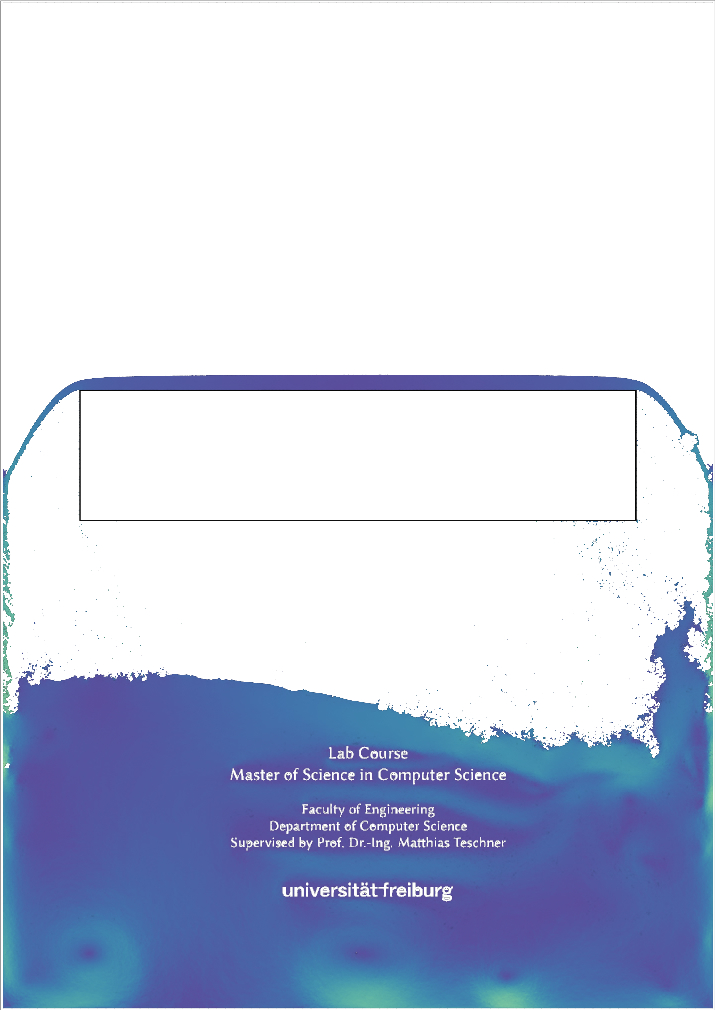
\includegraphics[width=\paperwidth,height=\paperheight]{images/title/titlesim.jpg}}
  \begin{center}
    \Huge\textbf{\@title}\\
    \vspace{0.5cm}
    \Large{\@author}\\
    \vfill
    \begin{figure*}[h!]
      \centering
      \resizebox{10cm}{!}{$\frac{D\vek{u}}{Dt} = \nu \Laplace \vek{u} -\frac{1}{\rho} \nabla p + \vek{F}^{ext}$}
      \caption*{The Navier-Stokes equation for incompressible flow. This tile page itself is used as a simulation domain in which this equation is solved, highlighting the solver's ability to handle complex boundary conditions and resolve details while maintaining low levels of compression (here: $\rho^{max}_{err}<0.1\%$ for $N>250k$ particles)}
      % \caption{Colour coded velocity field of a simulation with 250000 particles, where the solver handles
      %   complex boundary conditions, turbulent flow at low viscosity and a pronounced free surface with less than
      %   0.1\% compression. \cite{ray-optics-book}}
      \label{fig:title-image}
    \end{figure*}
    \vfill
    \Large
    % \contour{black}{\textcolor{white}{Lab Course}}\\
    % \contour{black}{\textcolor{white}{Master of Science in Computer Science}}\\

    \vspace{5.2cm}
    % \vspace{0.5cm}
    % \large
    % Faculty of Engineering\\
    % Department of Computer Science\\
    % Supervised by Prof. Dr.-Ing. Matthias Teschner\\
    % \vspace{0.5cm}
    % % \includegraphics*[width=5cm]{images/title/ufr-?logo.png}
  \end{center}
\end{titlepage}
% \captionsetup[figure]{font=normalsize,labelfont=normalsize}

\tableofcontents
\newpage


\chapter{Introduction}
\chapter{Governing Equations of Fluid Flow}\label{chp:governing-equations}
In an attempt to create a numerical solver for fluid dynamics problems, the governing equations of the underlying physical process must first be understood and formulated. Only then can an appropriate discretization be applied to numerically solve for desired properties of a system. In this chapter, the abstractions of continuum mechanics are used as a framework to describe incompressible flow. Physical principles such as conservation of mass and momentum are used to derive the continuity and momentum equations which encode them, then augmented by constitutive relations which describe properties of Newtonian fluids to finally yield the Navier-Stokes equations as governing equations.
\autocite*{anderson}\autocite*{tutorial}

The particular form of these equations will favour a Lagrangian view of the system, in which the frame of reference in which quantities are described is advected along with the flow of the fluid itself, which will seamlessly integrate with the discretization scheme later used to derive workable numerical algorithms.



\section{Lagrangian and Eulerian Continuum Mechanics}
The purpose of our mathematical modelling of fluids is to simulate fluid dynamics at macroscopic scales with numerical methods. We know that fluids consist of innumerable molecules, and smaller particles yet, interacting in complex ways, which give rise to emergent properties that we observe on a macroscopic scale. Instead of resolving all scales and simulating from quantum mechanical principles up, we content with modelling the emergent properties themselves, focusing on the question of how fluids behave on our desired scales instead of what gives rise to such effects. Our macroscopic scale is so many orders of magnitude larger than the quantized world of particles, that we can reasonably assume quantities describing the fluid to be continuous and tackle them with the tools of calculus. This gives rise to the field of \emphasis{Continuum Mechanics}.\\
In the following derivations, two major points of view can be taken, which produce different but equivalent forms of equations: the Eulerian or conservation forms, and the Lagrangian or nonconservation forms of the equations\autocite*{anderson}.

Using the assumption from continuum mechanics that quantities of our fluid are continuously distributed in space and asserting that they be differentiable, we can define derivatives on them. The two major forms of equations arise from a different interpretation of the so-called substantial derivative\autocite*{anderson} or material derivative\autocite*{tutorial} $\frac{D}{Dt}$. This operator describes the instantaneous time rate of change of a quantity of a continuum element as it moves through space \autocite*{anderson}. This movement through space however can be observed from different frames of reference:
\begin{itemize}
    \item a frame that is advected along with the flow of the fluid, in which the continuum element observed appears unmoving
    \item a frame that is unmoving in space and located at a fixed point, observing the flow of the fluid as continuum elements move through it
\end{itemize}

For both frames of reference, it can be derived that the material derivative in vector notation is \autocite*{anderson}:

\begin{align}
    \frac{D}{Dt} = \underbrace{\frac{\partial }{\partial t}}_{\text{local derivative}} + \underbrace{(\vek{v}\cdot \nabla)}_{\text{convective derivative}}
\end{align}
where $\vek{v}$ is the velocity of the element and $\nabla$ denotes the differential operator $\left(\frac{\partial}{\partial x_0}, \frac{\partial}{\partial x_1}, \dots,  \frac{\partial}{\partial x_n}\right)^T$ in $n$ dimensions \autocite*{anderson}. If an Eulerian view is chosen, there is an additional term for the convective derivate, which describes a rate of change of a quantity at a fixed point due to movement of the fluid. If a Lagrangian view is taken, the reference frame is advected with the velocity $\vek{v}$, precisely such that the convective derivative is zero and the material derivative simply becomes the total time derivative of a quantity. The difference between the two views is illustrated in \autoref{fig:lagrange-euler-1d}. In a way, the Lagrangian frame of reference is chosen precisely such that only local derivatives suffice to describe material derivatives by using a coordinate transformation defined by the velocity field.

How this simpler, Lagrangian form can be used largely depends on the later choice of discretization: discretizing space and tracking the fluid that moves through it favours an Eulerian framework, while discretizing the continuum into particles and sampling quantities only at advected particle positions makes the Lagrangian view convenient.\\
As is common for SPH discretizations, we will elect the Lagrangian view since it not only harmonizes well with particle-based discretizations but holds additional desirable properties such as making conservation of mass trivial to implement and enabling solving the Navier-Stokes equations for primitive quantities instead of flux quantities that may cause drift instead of oscillations due to numerical inaccuracy. We state all following equations in the Lagrangian, nonconservation form.

\begin{figure}
    \begin{center}
        \begin{subfigure}[t]{0.5\textwidth}
            \centering
            \begin{asy}
                import graph;
                defaultpen(fontsize(8pt));
                size(7cm,0);
                real xmin = -3;
                real xmax = 3;
                real ymin = 0;
                real ymax = 3;

                real b(real x) {return x < -0.7?0:(x>0.7?0:ymax);}
                real f(real x) {
                        real t = 0.3;
                        real sum = 0;
                        int n = 100;
                        real dx = 2.0 / n;
                        for (int i = 0; i <= n; ++i) {
                                real xi = -1 + i * dx;
                                sum += exp(-((x - xi) * (x - xi)) / (4 * t)) * b(xi);
                            }
                        return sum / (sqrt(4 * 3.141592653589793 * t)) * dx;
                    }

                draw((0, b(0)) .. (0, f(0)), black, arrow=Arrows(TeXHead));
                label("local",(0,(b(0)-f(0))/2.+ f(0)), E);

                draw(graph(new real(real x) { return b(x); },xmin,xmax, n=1000), heavyblue);
                draw(graph(new real(real x) { return f(x); },xmin,xmax, n=1000), lightblue+dashed);
                label("$A(\vek{x},t)$",(-0.69, b(-0.69)),NW, heavyblue);
                label("$A(\vek{x},t+\Delta t)$",(2.0, f(2.0)),NE, lightblue);

                // draw axis
                arrowbar axisarrow = Arrow(TeXHead);
                draw((xmin,0) -- (xmax,0), arrow=axisarrow);
                label("$x$",(xmax,0),S);
                draw((xmin+0.5,ymin) -- (xmin+0.5,ymax+0.5), arrow = axisarrow);
                label("$A$",(xmin+0.5,ymax+0.5),E);

                draw((0,ymin) -- (0,ymax+0.5),  black+dotted);
                dot("$\vek{x}_i$",(0,ymin),S);
            \end{asy}
            \caption{Lagrangian view}
        \end{subfigure}%
        ~
        \begin{subfigure}[t]{0.5\textwidth}
            \centering
            \begin{asy}
                import graph;
                defaultpen(fontsize(7.5pt));
                size(7cm,0);
                real xmin = -3;
                real xmax = 3;
                real ymin = 0;
                real ymax = 3;

                real b(real x) {return x < -0.7?0:(x>0.7?0:ymax);}
                real f(real x) {
                        real t = 0.3;
                        real sum = 0;
                        int n = 100;
                        real dx = 2.0 / n;
                        for (int i = 0; i <= n; ++i) {
                                real xi = -1 + i * dx;
                                sum += exp(-((x - xi) * (x - xi)) / (4 * t)) * b(xi);
                            }
                        return sum / (sqrt(4 * 3.141592653589793 * t)) * dx;
                    }

                draw((0, b(0)) .. (0, f(0)), black, arrow=Arrows(TeXHead));
                draw((-0.6, f(0)) .. (0.6, f(0)), black+dotted);
                label("local",(0,(b(0)-f(0))/2.+ f(0)), W);
                draw((0, f(0)) .. (0, f(-0.6)), black, arrow=Arrows(TeXHead));
                label("convective",(0,(f(0)-f(-0.6))/2.+ f(-0.6)), W);

                draw(graph(new real(real x) { return b(x+0.6); },xmin,xmax, n=1000), heavyblue);
                draw(graph(new real(real x) { return f(x-0.6); },xmin,xmax, n=1000), lightblue+dashed);
                label("$A(\vek{x},t)$",(-0.69-0.6, b(-0.69)),NW, heavyblue);
                label("$A(\vek{x},t+\Delta t)$",(2.0, f(2.0)+0.2),NE, lightblue);

                // draw axis
                arrowbar axisarrow = Arrow(TeXHead);
                draw((xmin,0) -- (xmax,0), arrow=axisarrow);
                label("$x$",(xmax,0),S);
                draw((xmin+0.5,ymin) -- (xmin+0.5,ymax+0.5), arrow = axisarrow);
                label("$A$",(xmin+0.5,ymax+0.5),E);

                draw((0,ymin) -- (0,ymax+0.5),  black+dotted);
                dot("$\vek{x}$",(0,ymin),S);
                dot("$\vek{x}_i(t)$",(-0.6,ymin),SW);
                dot("$\vek{x}_i(t+\Delta t)$",(0.6,ymin),SE);
            \end{asy}
            \caption{Eulerian view}
        \end{subfigure}
    \end{center}
    \caption{A field quantity $A$ in one dimension is shown at some time $t$ and a later time $t+\Delta t$ where the distribution of $A$ has changed due to some diffusive process and the quantity was advected in positive $x$-direction. In the Lagrangian view, changes in a quantity $A$ are evaluated at the advected position $\vek{x}_i$ at any point in time and only the local derivative is needed to describe the change in $A$ at $\vek{x}$. In the Eulerian view there are two reasons for $A$ at a point $\vek{x}$ fixed in space to change: the local derivative due to the diffusive process and the convective derivative due to the advection of the quantity with the velocity field.}
    \label{fig:lagrange-euler-1d}
\end{figure}

\section{The Continuity Equation}\label{sec:continuity-equation}
Using the Lagrangian view of continuum mechanics, we can apply laws of conservation to derive equations that express invariants of each fluid element with respect to time, which is an important step towards describing the dynamics of the system as time evolves. One such equation is the \emphasis{continuity equation}, which expresses conservation of mass:\\
Consider an infinitesimally small volume element $\delta \mathcal{V}$ with density $\rho$. The mass of the volume $\delta m$ is simply\autocite*{anderson}:
\begin{equation}\delta m = \rho \delta\mathcal{V}\label{eq:infintitesimal_volume}\end{equation}
and is invariant under the material derivative in the Lagrangian reference frame \autocite*{anderson}:
\begin{align}
    \frac{D\delta m}{D t} & = 0                                                                                                 & \textit{conservation of mass}                    \\
                          & = \frac{D \rho \delta\mathcal{V}}{Dt}                                                               & \textit{identity \ref{eq:infintitesimal_volume}} \\
                          & = \delta\mathcal{V} \frac{D \rho}{Dt} + \rho \frac{D \delta\mathcal{V}}{Dt}                         & \textit{product rule of calculus}                \\\label{eq:cont-eq-unfinished}
                          & =  \frac{D \rho}{Dt} + \rho \left(\frac{1}{\delta\mathcal{V}} \frac{D \delta\mathcal{V}}{Dt}\right) & \textit{divide by $\delta \mathcal{V}$}
\end{align}

We can now apply the \emphasis{divergence theorem} to relate $\frac{D\mathcal{V}}{D t}$ to the divergence of the velocity across the volume of the element, where $\partial \mathcal{V}$ is its surface and $\vek{n}$ the corresponding unit normal vector \autocite*{anderson}:

\begin{equation}\label{eq:div-theorem}
    \frac{D\mathcal{V}}{D t} =
    \oint_{\partial \mathcal{V}} \vek{v} \cdot \vek{n}\, dS =
    \int_{\mathcal{V}} \left( \nabla\cdot \vek{v}\right)\,d\mathcal{V}
\end{equation}

As the volume $\mathcal{V}$ approaches the infinitesimal volume element $\delta \mathcal{V}$ of interest, the velocity in the volume becomes constant, the integral vanishes, and it holds that \autocite*{anderson}:


\begin{equation}\label{eq:div-theorem-on-dV}
    \frac{D(\delta \mathcal{V})}{D t} = \left( \nabla\cdot \vec{v}\right) \delta \mathcal{V}
\end{equation}

Substituting \autoref{eq:div-theorem-on-dV} into \autoref{eq:cont-eq-unfinished} we finally obtain the continuity equation:

\begin{equation}\label{eq:continuity-eq}
    \text{\fbox{$\frac{D\rho}{D t} + \rho\left( \nabla \cdot \vek{v} \right) = 0$}}
\end{equation}

This is one of the Navier-Stokes equations in its derivative form, as opposed to the more general integral form \autocite*{anderson}. When we additionally assume that the fluid is incompressible across a wide range of pressures, as is often done when simulating hydrodynamics, we can assert that the density of the fluid element in a Lagrangian reference frame is constant, meaning:
\begin{equation}\label{eq:continuity-means-density-dt-zero}
    \frac{D\rho}{D t} = 0
\end{equation}
and therefore the velocity field of the flow for constant density is divergence-free\autocite*{continuum-intro}:
\begin{equation}\label{eq:continuity-means-velocity-divergence-zero}
    \nabla\cdot \vek{v} = 0
\end{equation}
In the following sections, the fluid will generally be assumed to be incompressible.\\

An alternative derivation of the continuity equation uses the \emphasis{Reynolds Transport Theorem}, which describes the material derivative of a scalar or tensor quantity $q(\vek{x}, t)$ integrated over a volume as the sum of its time rate of change within the volume and the flux of the quantity through the volume's surface \autocite*{continuum-intro}:
\begin{equation}\label{eq:reynolds-transport-theorem}
    \frac{D}{D t}\int_\mathcal{V} q(\vek{x}, t)\,dV = \int_\mathcal{V} \frac{\partial q(\vek{x}, t)}{\partial t} \,dV + \oint_{\partial\mathcal{V}}  q(\vek{x}, t)(\vek{v} \cdot \vek{n})\,dS
\end{equation}

This derivation goes as follows \autocite*{continuum-intro}:

\begin{align}
    0 & = \frac{D}{Dt} \int_\mathcal{V}\rho\,dV                                                                                & \textit{conservation of mass}                   \\
      & = \int_\mathcal{V} \frac{\partial\rho}{\partial t} \,dV + \oint_{\partial \mathcal{V}} \rho (\vek{v}\cdot\vek{n}) \,dS & \textit{Reynolds Transport Theorem}             \\
      & = \int_\mathcal{V} \frac{\partial\rho}{\partial t} \,dV + \int_{\mathcal{V}} \nabla \cdot (\rho \vek{v}) \,dV          & \textit{Divergence Theorem}                     \\
      & = \int_\mathcal{V} \left(\frac{\partial\rho}{\partial t} + \nabla \cdot (\rho \vek{v})\right) \,dV                     & \textit{combine integrals}                      \\
      & = \int_\mathcal{V} \left(\frac{D\rho}{D t} + \rho \nabla \cdot  \vek{v}\right) \,dV                                    & \textit{constant density, Lagrangian framework} \\
      & \overset{\forall\mathcal{V}}{\Longrightarrow} \frac{D\rho}{D t} + \rho \left(\nabla \cdot  \vek{v}\right) = 0          & \textit{integral holds for all $\mathcal{V}$}
\end{align}

This use of the Reynolds Transport Theorem is very similar to the derivation that follows in \autoref{sec:momentum-equation}, which is why this alternative derivation was stated.

\section{The Cauchy Momentum Equation}\label{sec:momentum-equation}

Mass is not the only conserved quantity that can be formulated in terms of a volume integral which can be transformed into a more convenient form using Reynolds Transport Theorem: a vital step in the derivation of the Navier-Stokes equations comes from applying the same concept to the conservation of momentum. In fact, the \emphasis{Cauchy momentum equation}, which is the general case of the more specific momentum equation used in the Navier-Stokes equations, can be derived similarly to \autoref{sec:continuity-equation}, additionally using the continuity equation itself and Newton's second law.

We begin by observing that the change of momentum of a fluid volume $\mathcal{V}$ can be defined as the material derivative of the momentum $\int_\mathcal{V}(\rho\vek{v})\,dV$ and simplify the resultant expression\autocite*{continuum-intro}:
\begin{align}
     & \frac{D}{Dt}\int_\mathcal{V}(\rho\vek{v})\,dV                                                                                                                    & \textit{define change in momentum}      \\ & = \int_\mathcal{V} \frac{\partial (\rho\vek{v})}{\partial t}\,dV + \oint_{\partial \mathcal{V}} \rho \vek{v} (\vek{v} \cdot \vek{n})\,dS & \textit{Reynolds Transport Theorem \ref{eq:reynolds-transport-theorem}} \\
     & = \int_\mathcal{V}\frac{D}{Dt}(\rho\vek{v})\,dV + \int_\mathcal{V} (\rho\vek{v} )\nabla\cdot\vek{v} \,dV                                                         & \textit{Divergence Theorem}             \\
     & = \int_\mathcal{V} \rho\frac{D\vek{v}}{Dt} + \vek{v}\frac{D\rho}{Dt} + (\rho\vek{v}) \nabla\cdot\vek{v} \,dV                                                     & \textit{product rule on first integral} \\
     & = \int_\mathcal{V} \rho\frac{D\vek{v}}{Dt} + \vek{v} \underbrace{\left( \frac{D\rho}{Dt} + \rho \nabla\cdot\vek{v} \right)}_{\text{continuity equation} =0} \,dV & \textit{factor out $\vek{v}$}           \\\label{eq:momentum-lhs}
     & = \int_\mathcal{V} \rho\frac{D\vek{v}}{Dt} \,dV
\end{align}

Then, we use Newton's second law, best known in its form $F=m\vek{a}$, to assert that this change in momentum $m\vek{a}$ is equal to the sum of forces exerted on the fluid volume, which can be decomposed into body forces $\vek{b}^{ext}$ per unit mass\autocite*{continuum-intro} that act on the entire fluid mass homogeneously 'at a distance'\autocite*{anderson}, like gravity for example, and into surface forces described by stress vectors $\vek{t}$ integrated over the fluid element's surface\autocite*{continuum-intro}:
\begin{equation}
    \int_\mathcal{V} \rho\frac{D\vek{v}}{Dt} \,dV = \oint_\mathcal{\partial V}\vek{t}\,dS + \rho\vek{b}^{ext}
\end{equation}
One can define the \emphasis{Cauchy stress tensor} $\mat{T}$ (sometimes referred to as $\mat{\sigma}$) for the material such that it satisfies\autocite*{continuum-intro} $\mat{T}\vek{n} = \vek{t}$. Then, the divergence theorem may be applied again and the total forces acting on the fluid element can be written as:
\begin{equation}\label{eq:momentum-total-forces}
    \int_\mathcal{V}\nabla\cdot\mat{T}\,dV + \rho\vek{b}^{ext}
\end{equation}

Setting the expressions for total force in \autoref{eq:momentum-total-forces} and total change of momentum in \autoref{eq:momentum-lhs} equal according to Newton's Law, we obtain:
\begin{align}
    \int_\mathcal{V}  \rho\frac{D\vek{v}}{Dt} - \nabla\cdot\mat{T} - \rho\vek{b}^{ext} \,dV = 0
\end{align}
From this, we have obtained the \emphasis{Cauchy Momentum Equation} as our equation of motion\autocite*{tutorial}:

\begin{equation}\label{eq:cauchy-momentum-eq}
    \text{\fbox{$\rho\frac{D\vek{v}}{Dt} =  \nabla\cdot\mat{T} + \rho\vek{b}^{ext}$}}
\end{equation}

\section{The Lagrangian Navier-Stokes Equations}
With the Cauchy momentum equation we have reached the end of what can be modelled using general physical principles and continuum mechanics and is valid for a range of materials. To close the system of equations for fluid flow, generality must be given up and specific assumptions about the behaviour of fluids must be used to model the specific stress tensor $\mat{T}$ representing incompressible, linearly viscous or Newtonian fluids. In order to derive the form of the tensor, we make the further assumptions about the fluid that will later be clarified:
\begin{enumerate}
    \item Fluids cannot sustain shear stresses when in rigid body motion.\label{enum:ns-fluid-cant-sustain-shear}
    \item Viscosity depends on the symmetric component of the gradient of velocity, it is linearly proportional to the rate of deformation tensor.\label{enum:ns-vis-prop-rate-of-deform}
\end{enumerate}


All remaining terms of the Cauchy momentum equation are clear, only the stress tensor $\mat{T}$ needs to be elaborated upon. First, it can be noted that $\mat{T}$ is a linear transformation\autocite*{continuum-intro} and that the tensor is symmetric\autocite*{continuum-intro}, as in equal to its transpose $\mat{T}^T = \mat{T}$ or $\mat{T}_{ij} = \mat{T}_{ji}$. This means that in three dimensions for example, only six degrees of freedom actually exist in this tensor\autocite*{incompressible-flow-volker}.

The element $\mat{T}_{ij}$ expresses a stress along some axis $\vek{e_i}$ acting on a plane perpendicular to $\vek{e_j}$, which means that the diagonal elements $\mat{T}_{ii}$ are normal stresses called \textit{tensile stresses} for negative values and \textit{compressive stresses} for positive values of $\mat{T}_{ii}$\autocite*{continuum-intro}, while $\forall i\neq j:\,\mat{T}_{ij}$ refer to \textit{shear stresses}\autocite*{anderson}.\\


To make this tensor more tractable, it can be assumed that a fluid is a material which cannot sustain shear stresses when in rigid body motion, including rest\autocite*{continuum-intro} (assumption \ref{enum:ns-fluid-cant-sustain-shear}) - this means that when in rigid body motion, the stress vector on any plane is normal to that plane\autocite*{continuum-intro}, the stress is therefore isotropic and $\mat{T}$ must be represented by the only isotropic second order tensor $\lambda\mat{\mat{1}}$ or $\lambda\delta_{ij}$ for some $\lambda\in\mathds{R}$ where $\delta_{ij}$ is the Kronecker delta\autocite*{course-notes-12800}. This motivates a decomposition of $\mat{T}$ for any general motion into a sum of an isotropic tensor describing \textit{volumetric stress} caused by pressure forces and the \textit{deviatoric stress} $\mat{V}$ which simply describes deviation of the total stress $\mat{T}$ from the volumetric stress\autocite*{derivation-ns-undergrad}:
\begin{align}\label{eq:stress-tensor-decomp}
    \mat{T} = \mat{V} -p\mat{1}
\end{align}
Conventionally, the pressure $p$ is defined such that a positive pressure causes a negative stress, meaning the pressure acts normal to the surface and is directed into the fluid volume $\mathcal{V}$\autocite*{incompressible-flow-volker}. For a fluid at rest $\mat{V}_{ij} = 0$ holds and the normal stress is isotropically $-p$ according to \textit{Pascal's law}\autocite*{course-notes-12800}. \autoref{eq:stress-tensor-decomp} decomposes stresses into a part caused by pressure and one caused by viscosity, which is why $\mat{V}$ is sometimes referred to as the \textit{viscous stress tensor}\autocite*{incompressible-flow-volker}. Viscosity can be thought of as internal friction in a fluid or its resistance to deformation. \\

The remaining term $\mat{V}$ is caused by viscosity and modelled according to assumption \ref{enum:ns-vis-prop-rate-of-deform} in terms of the gradient of the velocity. This makes intuitive sense: where the velocity is homogeneous, and the gradient is zero, there is no friction between fluid elements - where the velocity differs greatly, there is more friction. Since velocity is a vector quantity, the gradient $\nabla\vek{v}$ is a tensor\autocite*{incompressible-flow-volker}:
\begin{equation}
    (\nabla \vek{v})_{ij} = \partial_j v_i = \frac{\partial v_i}{\partial x_j}
\end{equation}
As always, we can decompose this tensor $\mat{L} := \nabla \vek{v} $ into a sum of a symmetric and an antisymmetric part \autocite*{continuum-intro}:
\begin{align}
    \mat{L} & = \mat{D} + \mat{W}                           \\
    \mat{D} & = \frac{1}{2}\left(\mat{L} + \mat{L}^T\right) \\
    \mat{W} & = \frac{1}{2}\left(\mat{L} - \mat{L}^T\right) \\
\end{align}

$\mat{D}$ is referred to as the \emphasis{rate of deformation tensor} and $\mat{W}$ is called the \emphasis{spin tensor}.\\


This decomposition is convenient since the spin tensor does not contribute to viscosity  and only the rate of deformation tensor may be focused on. Note that since the deviatoric stress $\mat{V}$ we are trying to approximate is symmetric, and it only makes sense to use the symmetric component of the velocity gradient to model it.

Intuitively, the spin tensor encodes the rotational component of the velocity gradient, and a steadily rotating fluid (where $\mat{D}_{ij}=0$) is like a rigid body rotation: the relative positions of the fluid elements do not change, only their orientation with respect to a fixed reference frame, and therefore there is no friction. There is a vector $\vek{\omega}$ such that for any $\vek{v}$ it holds that $\mat{W}\vek{v} = \vek{\omega} \times \vek{v}$, where $\vek{\omega}$ points in the axis of rotation with a length of the angular velocity \autocite*{continuum-intro}. This is why the spin tensor is closely related to the vorticity tensor $2\mat{W}$\autocite*{continuum-intro}. In fact, enforcing that viscosity shall not affect the rotational component of velocity gradients and preserving accurate vorticity is key to accurately simulating turbulences in incompressible flows and conserving angular momentum \autocite*{vorticity-micropolar}.

Focusing further on the rate of deformation tensor, assumption \ref{enum:ns-vis-prop-rate-of-deform} can now fully be appreciated. One defining characteristic of Newtonian fluids is the assumption dating back to Isaac Newton that viscosity depends \textit{linearly} on the rate of deformation tensor \autocite*{anderson}. This means that terms of an order higher than linear may be neglected for small velocity gradients\autocite*{incompressible-flow-volker} and constant terms cannot occur since shear stress is only proportional to the rate of deformation, not deformation itself\autocite*{continuum-intro}: if a shear stress is applied to a fluid it will eventually continuously deform at some non-zero rate but will remain in that deformed state if the stress is removed, unlike purely elastic materials\autocite*{continuum-intro}. In other words $\mat{V}$ must vanish when the velocity is homogeneous since there is no friction in that case \autocite*{incompressible-flow-volker}.

We now know that for incompressible fluids $\mat{V}$ is of the form \autocite*{incompressible-flow-volker}:
\begin{align}
    \mat{V} & = 2\mu \mat{D}+ \lambda (\nabla\cdot\vek{v})\mat{1}                                                                                                  \\
            & = \frac{2\mu}{2}\left((\nabla \vek{v}) + (\nabla \vek{v})^T\right) + \underbrace{\lambda (\nabla\cdot\vek{v})\mat{1}}_{\text{incompressibility = 0}} \\
            & = \mu\left((\nabla \vek{v}) + (\nabla \vek{v})^T\right)
\end{align}
where $\mu$ is the dynamic viscosity\autocite*{anderson} or first-order viscosity\autocite*{incompressible-flow-volker}. A second-order viscosity $\lambda$ exists for compressible flows\autocite*{anderson}, but can be neglected here.

Combining the deviatoric stress with the volumetric stress, the \emphasis{constitutive relation} for the stress tensor $\mat{T}$ of an incompressible, Newtonian fluid is finally obtained\autocite*{tutorial}:
\begin{equation}\label{eq:consistutive-relation}
    \text{\fbox{$\mat{T} = -p\mat{1} + \mu\left((\nabla \vek{v}) + (\nabla \vek{v})^T\right)$}}
\end{equation}

With the constitutive relation in hand, the Cauchy momentum equation can be revisited, and \autoref{eq:consistutive-relation} can be inserted into \autoref{eq:cauchy-momentum-eq}:
\begin{align}
    \label{eq:ns-deriv-step-1}\rho\frac{D\vek{v}}{Dt} & =  \nabla\cdot\left(-p\mat{1} + \mu\left((\nabla \vek{v}) + (\nabla \vek{v})^T\right)\right) + \rho\vek{b}^{ext}                                                         & \textit{insert Eq. \ref{eq:consistutive-relation} into Eq. \ref{eq:cauchy-momentum-eq}} \\
    \label{eq:ns-deriv-step-2}\rho\frac{D\vek{v}}{Dt} & = \nabla\cdot (-p\mat{1}) + \mu\nabla\cdot\left((\nabla \vek{v}) + (\nabla \vek{v})^T\right)+\rho\vek{b}^{ext}                                                           & \textit{$\nabla\cdot$ is linear}                                                        \\
    \label{eq:ns-deriv-step-3}\frac{D\vek{v}}{Dt}     & = -\frac{1}{\rho}\nabla p + \nu\nabla\cdot\left((\nabla \vek{v}) + (\nabla \vek{v})^T\right)+\vek{b}^{ext}                                                               & \textit{$\nabla\cdot (-p\mat{1}) = -\nabla p$, divide by $\rho$}                        \\
    \label{eq:ns-deriv-step-4}\frac{D\vek{v}}{Dt}     & = -\frac{1}{\rho}\nabla p + \nu\left(\underbrace{\nabla\cdot(\nabla \vek{v})}_{=\Laplace\vek{v}} + \underbrace{\nabla\cdot(\nabla \vek{v})^T}_{=0} \right)+\vek{b}^{ext} & \textit{$\nabla\cdot$ is linear}                                                        \\
    \label{eq:ns-deriv-step-5}\frac{D\vek{v}}{Dt}     & = -\frac{1}{\rho}\nabla p + \nu\Laplace\vek{v}+\vek{b}^{ext}                                                                                                             &
\end{align}

A few things of note happen in this derivation:
\begin{itemize}
    \item The kinematic viscosity $\nu$ is defined as $\frac{\mu}{\rho}$ and inserted in \autoref{eq:ns-deriv-step-3}
    \item The identity $\nabla\cdot(-p\mat{1}) = -\nabla\cdot\begin{bmatrix}
                  p & 0 & 0 \\
                  0 & p & 0 \\
                  0 & 0 & p \\
              \end{bmatrix} = -\begin{bmatrix}
                  \sfrac{\partial p}{\partial x} \\
                  \sfrac{\partial p}{\partial y} \\
                  \sfrac{\partial p}{\partial y} \\
              \end{bmatrix} = -\nabla p$ is used in \autoref{eq:ns-deriv-step-3}.
    \item For sufficiently smooth $\vek{v}$ and $\nabla\cdot\vek{v}=0$ one can show using the Theorem of Schwarz that $\nabla\cdot(\nabla \vek{v})=\Laplace\vek{v}$ as annotated in \autoref{eq:ns-deriv-step-4}\autocite*{incompressible-flow-volker}.
    \item Similarly, in \autoref{eq:ns-deriv-step-4} $\nabla\cdot(\nabla\vek{v}^T) = \nabla(\nabla\cdot\vek{v}) =0$ is used\autocite*{incompressible-flow-volker}, since the continuity equation for fluids of homogeneous density implies $\nabla\cdot\vek{v}=0$.
\end{itemize}

With all this, the final Navier-Stokes momentum equation for incompressible Newtonian fluids in Lagrangian form is obtained in step \ref{eq:ns-deriv-step-5}:

\begin{equation}\label{eq:navier-stokes-momentum}
    \text{\fbox{$\frac{D\vek{v}}{Dt}=-\frac{1}{\rho}\nabla p+\nu\Laplace\vek{v}+\vek{b}^{ext}$}}
\end{equation}

\section{Equations of State}

Although the momentum equation typically takes centre stage when discussing the Navier-Stokes equations, it is important to realize that the complete Navier-Stokes equations actually refer to a set of equations and the momentum equation cannot function on its own. At the very least, the continuity equation should be included, sometimes accompanied by an energy balance equation which is crucial to heat transport problems and formulates conservation of energy in viscous flows\autocite*{anderson}. For the dynamics of the systems considered here, the continuity and momentum equations appear to be sufficient, but one field quantity remains elusive until now: We have yet to discuss how to compute pressure.\\


When incompressibility is strongly enforced, the continuity equation is a constraint on the momentum equation that $p$ can be chosen to fulfil, making it a Lagrange multiplier to the equation\autocite*{tutorial}. Since strongly enforced incompressibility generally requires solving a system to solve the Poisson equation for pressure and can be more involved, a more straightforward first approach is to employ an \emphasis{Equation of State} to couple pressure to known quantities. Such an equation of state can be thought of intuitively as relating strain and stress, or a deformation of a material and the potential caused by this deformation, the negative gradient of which is a force. In this case a deviation of the fluid from its rest density $\rho_0$ or volume $V_0$ causes a pressure potential, the negative gradient of which is a pressure force that counteracts the deformation, in this case compression, as demonstrated in the hydrostatic case.\\


There are many such equations of state to choose from. While this choice indeed encodes different physical assumption about the fluid, the choice often appears to be motivated by implementation details and practical reasons rather than general physical principles. The equation of state should be chosen with the goal of low compressibility and well-behavedness of the system in mind and options include:


\begin{enumerate}
    \item $p = k\rho$ or $p=k(\rho-\rho_0)$ from the ideal gas equation \autocite*{wcsph}
    \item\label{enum:eos-murnaghan} $p=k\left(\frac{\rho}{\rho_0}-1\right)^\gamma$ which is sometimes referred to as Tait's equation\autocite*{wcsph}, while others critique this attribution to Tait\autocite*{moanghan-2012-sph-and-its-diverse-applications} and some refer to it as a form of the Murnaghan equation of state\autocite*{macdonald-state-equations-murnaghan} or attribute its first use to Kirkwood\autocite*{macdonald-state-equations-murnaghan}
    \item\label{enum:eos-clamping} $p=\max\left(0, k(\rho-\rho_0)\right)$ or $p=\max\left(0, k\left(\frac{\rho}{\rho_0}-1\right)^\gamma\right)$ to prevent negative pressure values\autocite*{tutorial}
\end{enumerate}

Option \ref{enum:eos-clamping} in particular is used to penalize relative deviations from rest density while preventing negative pressure values that may cause undesired clumping artefacts when using SPH discretizations. In the implementation used for this report, the equation:
\begin{equation}\label{eq:state-equation}
    p=\max\left(0, k\left(\frac{\rho}{\rho_0}-1\right)\right)
\end{equation}
was chosen by inserting $\gamma=1$ into option \ref{enum:eos-murnaghan} and applying clamping.


While the equation of state does allow the computation of the unknown pressure, it does not appear to help close the Navier-Stokes equations, since the problem was only pushed back to the seemingly arbitrary choice or some parameter $k$ representing stiffness. It is important to note that this parameter does not however govern the magnitude of pressure per se, but only the compressibility of the fluid\autocite*{tutorial}, where larger values of $k$ yield higher incompressibility but also higher pressure accelerations and therefore demand a higher resolution of time discretization to remain numerically stable\autocite*{tutorial} and satisfy the Courant-Friedrichs-Lewy condition\autocite*{pcisph}, decreasing computational efficiency. In order to ensure that the assumption of incompressibility made in the derivation of the Navier-Stokes momentum equations hold, a sufficiently large stiffness $k$ should be chosen for a given setting, such that compressibility becomes negligible.

Approximations for the choice of $k$ in Murnaghan's equation such as $k\approx \frac{\rho_0 c_s}{\gamma}$ exist, where $c_s$ is the speed of sound and relates to the speed of flow $\vek{v}_f$ \autocite*{wcsph}. Other methods such as Predictive-Corrective Incompressible SPH (PCISPH for short) approximate a globally constant $k$ specifically for SPH discretizations such that a more optimal trade-off of incompressibility and time step size might be realized. Generally, $k$ might need to be tuned depending on the simulated scenario in a fluid solver employing an equation of state.





\chapter{Smoothed Particle Hydrodynamics Discretization}\label{chp:sph-discretization}
\section{Kernel Functions}
\section{Discretizations and Properties}

\chapter{Solving for Incompressibility}
\section{Weakly Compressible SPH}
\section{Operator Splitting and Iterative Solver}

\chapter{Boundary and Initial Conditions}
\section{Non-Uniform Single Layer Boundaries}
\section{Jittered Initialization and Lattices}
\section{Solving for Equilibrated Density}


\chapter{Analysis}
\section{Oscillation Frequency and Error as a Function of Speed of Sound}
\section{Stability as a Function of Viscosity, Stiffness and Timestep}
\section{Stability over Viscosity and Stiffness}

\chapter{Conclusion}



\printbibliography[
  heading=bibintoc,
  title={Bibliography}
]
\end{document}